%!Tex Program = xelatex
\documentclass[a4paper]{book}

% 设置页边距
\usepackage{geometry}
\geometry{left=2cm, right=2cm, top=2.5cm, bottom=1cm}

% 中文断行
\XeTeXlinebreaklocale "zh"
\XeTeXlinebreakskip = 0pt plus 1pt

%% code include by PythonShell
%% From http://tex.stackexchange.com/questions/140923/how-to-automatically-align-the-four-choices-of-a-multiple-choice-question-in-exa
%% thanks to the author ollydbg23 @ stackexchange
%% some tiny modifies from PythonShell
%% 2014-01-08

\usepackage{ifthen}
\usepackage{calc}
\setlength\parindent{0pt}

    %usage \choice{ }{ }{ }{ }
    %(A)(B)(C)(D)
    \newcommand{\fourch}[4]{
	%\par
            \begin{tabular}{*{4}{@{}p{0.23\textwidth}}}
            [A] ~#1 & [B] ~#2 & [C] ~#3 & [D] ~#4
            \end{tabular}
    }

    %(A)(B)
    %(C)(D)
    \newcommand{\twoch}[4]{
	%\par
            \begin{tabular}{*{2}{@{}p{0.46\textwidth}}}
            [A] ~#1 & [B] ~#2
            \end{tabular}
    \par
            \begin{tabular}{*{2}{@{}p{0.46\textwidth}}}
            [C] ~#3 & [D] ~#4
            \end{tabular}
    }

    %(A)
    %(B)
    %(C)
    %(D)
    \newcommand{\onech}[4]{
	%\par
            [A] ~#1 \par [B] ~#2 \par [C] ~#3 \par [D] ~#4
    }

    \newlength\widthcha
    \newlength\widthchb
    \newlength\widthchc
    \newlength\widthchd
    \newlength\widthch
    \newlength\tabmaxwidth

    \setlength\tabmaxwidth{0.96\textwidth}
    \newlength\fourthtabwidth
    \setlength\fourthtabwidth{0.24\textwidth}
    \newlength\halftabwidth
    \setlength\halftabwidth{0.48\textwidth}

    \newcommand{\choice}[4]{
            \settowidth\widthcha{AM.#1}\setlength{\widthch}{\widthcha}
            \settowidth\widthchb{BM.#2}    
            \ifthenelse{\widthch<\widthchb}{\setlength{\widthch}{\widthchb}}{}
            \settowidth\widthchb{CM.#3}    
            \ifthenelse{\widthch<\widthchb}{\setlength{\widthch}{\widthchb}}{}
            \settowidth\widthchb{DM.#4}    
            \ifthenelse{\widthch<\widthchb}{\setlength{\widthch}{\widthchb}}{}     
            \ifthenelse{\widthch<\fourthtabwidth}{\fourch{#1}{#2}{#3}{#4}}
                               {\ifthenelse{\widthch<\halftabwidth\and\widthch>\fourthtabwidth}{\twoch{#1}{#2}{#3}{#4}}
                               {\onech{#1}{#2}{#3}{#4}}}
    }

\usepackage{fontspec}
\setmainfont{SimSun}	% 设置正文默认字体为SimSun

\newcommand\fontnamekai{楷体}	% 设置楷体
\newfontinstance\KAI {\fontnamekai}
\newcommand{\kai}[1]{{\KAI#1}}

\newcommand\fontnamehei{黑体}	% 设置黑体
\newfontinstance\HEI{\fontnamehei}  
\newcommand{\hei}[1]{{\HEI#1}} 

% 设置页眉
\pagestyle{myheadings}
\markboth{PythonShell 工作室}{2012年考研政治试题}

% 取消缩进
\setlength{\parindent}{0pt}

\begin{document}
\hei{一、单项选择题:}\kai{1~16小题,每小题1分,共16分。下列每题给出的四个选项中,只有一个选项是符合题目要求的。请在答题卡上将所选项的字母涂黑。}

\vspace{6pt}

%% Content from http://zhenti.kaoyan.eol.cn/
%% Format by PythonShell
%% 2014-01-08

\qquad People are, on the whole, poor at considering background
information when making individual decisions. At first glance this
might seem like a strength that \underline{\quad 1\quad} the
ability to make judgments which are unbiased by
\underline{\quad 2\quad} factors. But Dr Simonton speculated that
an inability to consider the big \underline{\quad 3\quad} was
leading decision-makers to be biased by the daily samples of
information they were working with. \underline{\quad 4\quad}, he
theorized that a judge \underline{\quad 5\quad} of appearing too
soft \underline{\quad 6\quad}crime might be more likely to send
someone to prison \underline{\quad 7\quad} he had already sentenced
five or six other defendants only to forced community service on
that day.

\qquad To \underline{\quad 8\quad} this idea, they turned their attention
to the university-admissions process. In theory, the \underline{\quad 9\quad} of an
applicant should not depend on the few others \underline{\quad 10\quad} randomly for interview during the same day, but Dr Simonton suspected the truth was \underline{\quad 11\quad}.

\qquad He studied the results of 9,323 MBA interviews \underline{\quad 12\quad} by 31 admissions officers. The interviewers had \underline{\quad 13\quad} applicants on a scale of one to five. This scale \underline{\quad 14\quad} numerous factors into consideration. The scores were \underline{\quad 15\quad} used in conjunction with an applicant's score on the Graduate Management Admission Test, or GMAT, a standardized exam which is \underline{\quad 16\quad} out of 800 points, to make a decision on whether to accept him or her.

\qquad Dr Simonton found if the score of the previous candidate in a daily series of interviewees was 0.75 points or more higher than that of the one \underline{\quad 17\quad} that, then the score for the next applicant would \underline{\quad 18\quad} by an average of 0.075 points. This might sound small, but to \underline{\quad 19\quad} the effects of such a decrease a candidate would need 30 more GMAT points than would otherwise have been \underline{\quad 20\quad}.

\vspace{6pt}

01. \choice{ grants  }{ submits  }{ transmits  }{ delivers}
02. \choice{ minor      }{  objective   }{ crucial       }{ external}
03. \choice{ issue      }{ vision      }{ picture       }{ moment}
04. \choice{ For example  }{ On average  }{ In principle  }{ Above all}
05. \choice{ fond       }{ fearful     }{ capable       }{ thoughtless}
06. \choice{ in         }{ on         }{ to            }{ for}
07. \choice{ if         }{ until       }{ though        }{ unless}
08. \choice{ promote       }{ emphasize   }{ share         }{ test}
09. \choice{ decision   }{ quality     }{ status        }{ success}
10. \choice{ chosen      }{ stupid     }{ found        }{ identified}
11. \choice{ exceptional  }{ defensible  }{ replaceable   }{ otherwise}
12. \choice{ inspired   }{ expressed   }{ conducted     }{ secured}
13. \choice{ assigned   }{ rated       }{ matched       }{ arranged}
14. \choice{ put        }{ got         }{ gave          }{ took}
15. \choice{ instead    }{ then        }{ ever          }{ rather}
16. \choice{ selected   }{ passed      }{ marked        }{ introduced}
17. \choice{ before      }{ after       }{ above         }{ below}
18. \choice{ jump       }{ float       }{ drop     }{ fluctuate}
19. \choice{ achieve    }{ undo        }{ maintain      }{ disregard}
20. \choice{ promising  }{ possible    }{ necessary     }{ helpful}

\hei{二、多项选择题:}\kai{17~33题,每小题2分,共34分。下列每题给出的四个选项中,至少有两个选项是符合题目要求的。请在答题卡上将所选项的字母涂黑。多选或少选均不得分。}

\vspace{6pt}

17. 马克思主义是关于无产阶级和人类解放的科学,实现共产主义是全人类解放的根本体现。人类解放包括
\begin{choices}
	\choice0 从自然的压迫下解放出来
	\choice0 从客观规律的制约下解放出来
	\choice0 从旧的社会关系的束缚下解放出来
	\choice0 从旧的传统观念的禁锢下解放出来
\end{choices}
18. 唯物史观第一次科学地解决了历史创造者的问题,认为人民群众是历史的创造者。人民群众
\begin{choices}
	\choice0 从量上说是指社会人的绝大多数
	\choice0 从质上说是对社会历史发展起推动作用的人们
	\choice0 在任何历史时期都不包括剥削阶级
	\choice0 最稳定的主体部分始终是从事物质资料生产的劳动群众及其知识分子
\end{choices}
19. 美国导演迈克尔。穆尔在他的最新记录片《资本主义:一个爱情故事》问世以来,一直颇受关注。“资本主义”为何与“爱情故事”联系起来呢?穆尔解释说,这是一种“贪欲之爱”,喜爱财富的人不仅爱他们自己的钱,也爱你口袋中的钱……很多人不敢说出它的名字,真见鬼,就说出来吧。这就是“资本主义”。对金钱的“贪欲”与资本主义连为一体,是因为
\begin{choices}
	\choice0 资本就是人格化的资本
	\choice0 赚钱体现了人的天然本性
	\choice0 资本的生命在于不断运动和不断增值
	\choice0 追逐剩余价值是资本主义生产方式的绝对规律
\end{choices}
20. 伴随着生产力发展,科技进步及阶级关系调整,当代资本主义社会的劳资关系和分配关系发生了很大变化。其中资本家及其代理人为缓和劳资关系所采取的激励制度有
\begin{choices}
	\choice0 职工终身雇佣制度
	\choice0 职工参与决策制度
	\choice0 职工选举管理着制度
	\choice0 职工持股制度
\end{choices}
21. 自第一个社会主义国家建立以来,社会主义事业的发展并不是一帆风顺的,社会主义发展道路的多样性以及发展过程中的前进性和曲折性的时间告诉我们
\begin{choices}
	\choice0 发展社会主义,不等于不学习西方资本主义的文明成果
	\choice0 坚持社会主义,不等于要坚持某种单一的社会主义模式
	\choice0 改革或抛弃某种社会主义模式,不等于改掉或抛弃社会主义
	\choice0 某种社会主义模式的失败,不等于整个社会主义事业的失败
\end{choices}
22. 党的十八大把科学发展观同马克思主义列宁主义、毛泽东思想、邓小平理论、“三个代表”重要思想一道确立为党必须长期坚持的指导思想。科学发展观是
\begin{choices}
	\choice0 中国特色社会主义理论体系的最新成果
	\choice0 中国革命、建设、改革经验的科学总结
	\choice0 指导党和国家全部工作的强大思想武器
	\choice0 中国共产党集体智慧的结晶
\end{choices}
23. 国务院新闻办公室发表的《西藏和平解放60年》白皮书指出,目前,西藏共有各类宗教活动场所1700余处,僧尼约4. 6万人,藏传佛教特有的活佛转世的传承方式得到充分尊重,寺庙学经、辩经、受戒、灌顶、修行等传统宗教活动和寺庙学经考核晋升学位活动正常进行,每年到拉萨朝佛敬香的信教群众达百万人次以上。上述事实表明,我国的宗教政策得到了充分贯彻。我国宗教政策主要有
\begin{choices}
	\choice0 尊重和保护公民的宗教信仰自由
	\choice0 积极引导宗教与社会
	\choice0 独立自主自办教会
	\choice0 依法管理宗教事务
\end{choices}
24. 统筹区域发展,促进区域协调发展,是我国经济社会发展的一个重点原则,坚持这一原则有利于
\begin{choices}
	\choice0 扩大内需,拉动经济增长
	\choice0 区域间优势互补,促进经济共同发展
	\choice0 不同区域人民共享改革发展成果
	\choice0 生产要素在区域间合理流动和配置
\end{choices}
25. 1992年初,邓小平在南方谈话中指出:“社会主义的本质是,解放生产,发展生产力。消除剥削,消除两极分化,最终达到共同富裕。“这一概括对社会主义传统认识的突破主要体现在
\begin{choices}
	\choice0 破除了脱离生产力水平抽象谈论社会主义的认识
	\choice0 否定了社会主义必须坚持公有制和按劳分配原则的认识
	\choice0 摆脱了长期以来忽视建设社会主义根本目的和目标的认识
	\choice0 Test
\end{choices}
26. PM2.5(细粒颗粒)这个大家原本很陌生的专有名词,因为2011年10月我国多地灰霾天气造成严重大气污染而迅速成为社会热词。2012年2月修订的《环境空气质量标准》增加了PM2.5指标,该指标随后又被写入政府工作报告。这既折射出当前我国环境污染的严重性,同时也反映了党和政府治理环境污染、建设生态文明的决心。十八大提出的生态文明建设新要求是
\begin{choices}
	\choice0 加大自然生态系统和环境保护力度
	\choice0 全面促进资源节约
	\choice0 优化国土空间开发格局
	\choice0 加强生态文明制度建设
\end{choices}
27. 1925至1927年的大革命规模宏伟,内涵丰富,与辛亥革命相比较,其不同点在于
\begin{choices}
	\choice0 它广泛而深刻地发动了工农群众
	\choice0 它的主要斗争形式是武装斗争
	\choice0 它的革命对象是帝国主义和封建军阀
	\choice0 它是在以国共合体为基础的统一战线的组织下进行的
\end{choices}
28.1931年1月至1935年1月,以王明为代表的“左”倾错误给中国革命带来严重危害,其主要错误有
\begin{choices}
	\choice0 排斥和打击中国民族资本主义势力
	\choice0 将反帝反封建与反资产阶级并列
	\choice0 集中力量攻打大城市
	\choice0 主张“一切经过统一战线”
\end{choices}
29. 抗日战争是近代以来中华民族反抗外敌入侵第一次取得完全胜利的民族解放战争,中国赢得抗日战争胜利的主要原因是
\begin{choices}
	\choice0 中国共产党发挥了中流砥柱的作用
	\choice0 中国的国力空前强大
	\choice0 得到了国际反法西斯力量的同情和支持
	\choice0 中国实现了空前的民族觉醒和民族团结
\end{choices}
30. 以毛泽东同志为核心的党的第一代中央领导集体带领全党全国和各族人民完成了新民主主义革命,进行了社会主义改造,确立了社会主义基本制度,这一基本制度的确立
\begin{choices}
	\choice0 为当代中国一切发展进步奠定了根本政治前提和制度基础
	\choice0 是中国历史上最深刻最伟大的社会变革
	\choice0 标志着马克思主义同中国实际第二次结合的完成
	\choice0 使广大劳动人民真正成为国家的主人
\end{choices}
31. 一位社会学家发现大楼的一块玻璃坏了,起初他没太当回事,没过多久,他发现许多处窗户都破损了,经过调研后,他得出结论:一样东西如果有点破损,人们就会有意无意地加快它的破损速度,一样东西如果完好无损,或是及时维护,人们就会精心的护理。这就是著名的“破窗定律”。下列关于道德修养的名言与“破窗定律”内涵相近的是
\begin{choices}
	\choice0 非知之难,行之惟难,非行之难,终之斯难。
	\choice0 善不可谓小而无益,不善不可谓小而无伤。
	\choice0 小善虽无大益,而不可不为。细恶虽无近祸,而不可不去。
	\choice0 见贤思齐焉,见不贤而内自省也。
\end{choices}
32. “可上九天揽月,可下五洋捉鳖”,2012年6月24日在航天员的手动操作下,我国“神航号”宇宙飞船与“天宫一号”交互对接成功,向未来建设宇宙空间站迈向坚实一步。就在同一天,我国的“蛟龙号”载人潜水器成功下潜7020米的深度,再次创造历史记录。这两次成就的里程碑意义在于
\begin{choices}
	\choice0 完成了“近地空间长期载人飞行”和“南海深部计划”
	\choice0 丰富了人类认识和开发宇宙的梦想和实践
	\choice0 为中国在太空和海底参与国际合体提供了更多机会
	\choice0 为中国在太空和大洋这两个尚未充分利用空间的活动创造了新可能性
\end{choices}
33. 2012年6.6至7日,上海合作组织成员国元首理事会第十二次会议在京举行。这是该组织发展进入第二个十年的首次峰会,与会各国元首就深化成员国友好合作以及重大国际和地区问题深入交换了意见,达成了新的重要共识。此次峰会的主要成果有
\begin{choices}
	\choice0 首次制定了中长期战略规划
	\choice0 签订了军事同盟条约
	\choice0 签署了首个人文合作宣言
	\choice0 增加了新的观察员国和对话伙伴国
\end{choices}
\vspace{6pt}

\hei{三、分析题:}\kai{34~38小题,第34小题12分,第35、36、37小题每题10分,第38小题8分,共50分。要求结合所学知识分析材料并回答问题。将答案写在答题纸指定位置上。}

\vspace{6pt}

\hei{34题、结合材料回答问题:}

\qquad \kai{华佗是我国东汉名医。一次,府吏倪寻和李延俩人均头痛发热。一同去请华佗诊治,华佗经过仔细的望色、诊脉,开出两付不同的处方。给倪寻开的是泻药,给李延开的是解表发散药。二人不解:我俩患的是同一症状,为何开的药方却不同呢?是不是华佗弄错了?于是,他们向华佗请教。华佗解释道:倪寻的病是由于饮食过多引起的,病在内,应当服泻药,将积滞泻去,病就好了。李延的病是受凉感冒引起的,病在外,应当吃解表药,风寒之邪随汗而去,头痛也就好了。你们病症相似,但病因相异,所以治之宜殊。二人拜服,回家后各自将药熬好服下,很快都痊愈了。}

\qquad \kai{中医是我国宝贵的医学遗产,强调辩证施治。华佗对症下药治头痛发热的故事含蕴丰富的辩证法思想。}

(1)指出其中所涉及的唯物辩证法基本范畴并分析其内涵。(6分)

(2)这个故事对我们理解“具体问题具体分析”有何启示?(4分)

\clearpage

\hei{35题、结合材料回答问题:}

\hei{材料1}

\begin{center}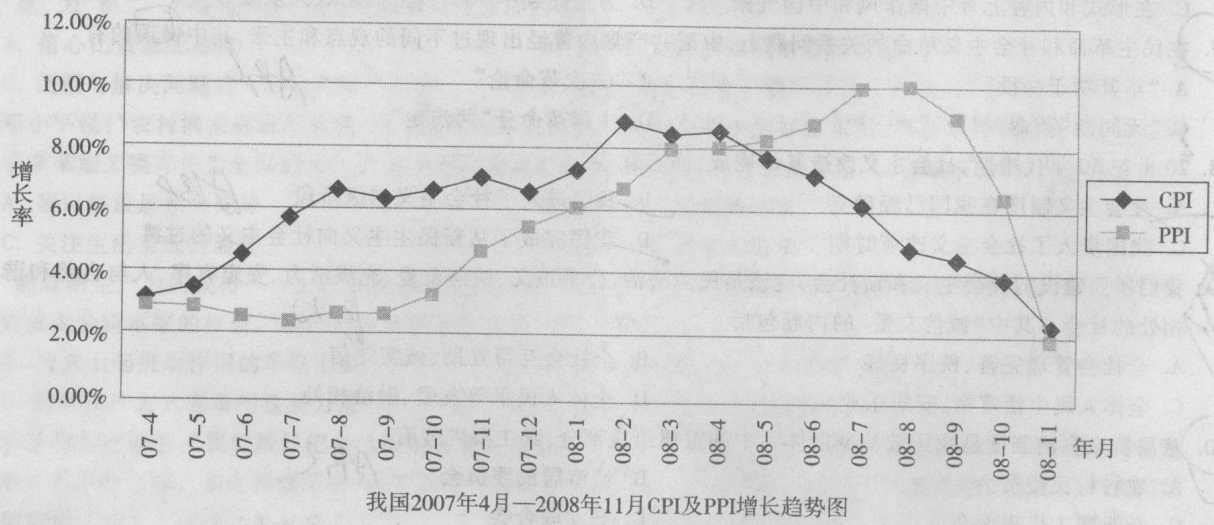
\includegraphics{35.jpg}\end{center}

\begin{center}我国2007年4月-2008年11月CPI及PPI增长趋势图\end{center}

\qquad \kai{注:CPI(消费价格指数)是反映一定时期内城乡居民家庭购买的生活消费品的价格和服务项目价格变动趋势和程度的相对数,一般认为CPI的增幅大于3%时,就存在通货膨胀的压力。PPI(生产价格指数)是衡量工业企业产品价格变动趋势和变动程度的指标。}

\begin{flushright}\kai{资料来源:国家统计局公布数据}\end{flushright}

\hei{材料2}

\qquad \kai{我国经济自2003年进入新一轮上升期,经济增长速度从2003年的10\%一路上涨,2006年突破11\%,并于2007达到11.9\%。然而经济偏快增长也带来一系列影响经济社会可持续发展的重大问题,经济增长有可能由偏快转为过热。2007年12月初召开的中央经济工作会议确定的宏观调控任务是:“防止经济增长由偏快转为过热,防止价格由结构性上涨演变为明显通货膨胀。”}

\qquad \kai{2008年,随着国际经济金融危机的不断加深,国内许多外向型出口企业经营出现困难,出口持续出现下滑势头。上半年经济增长开始放缓,GDP同比增长10.4\%,比去年同期回落1.8\%,上半年居民消费价格水平上涨7.9\%,这表明“防过热”已见效,但物价涨幅较高仍未得到有效控制。2008年7月25日召开的中央政治局会议明确了下半年经济工作的任务:把保持经济平稳较快发展,控制物价过快上涨放在突出的位置,即“一保一控”。财政部等部门宣布自2008年8月1日起提高部分出口商品的退税率,央行8月初调整了商业银行信贷规模,9月16日起又下调了人民币贷款基准利率和中小金融机构人民币存款准备金率,以缓解中小企业融资难、担保难以及流动资金短缺等问题。}

\qquad \kai{2008年前三季度,我国经济增速同比回落了2.3个百分点,经济增长五年多首次低于10\%,随着国际经济金融危机对我国实体经济影响日益显现,国内经济的下行风险逐步加大,中国已经从持续升温转入降温状态。11月9日国务院宣布实行积极的财政政策和适度宽松的货币政策,特别是拉动内需十项新举措的公布。释放出“保增长”的强烈信号,四万亿的投资将对经济产生最直接的拉动。十二月中央经济工作会议进一步明确指出必须把保持经济平稳较快发展作为明年经济工作的首要任务。要着力在保增长上下功夫,把扩大内需作为保增长的根本途径,把加快发展方式转变和结构调整作为保增长的主攻方向。把深化重点领域和关键环节改革,提高对外开放水平作为保增长的强大动力,把改善民生作为保增长的出发点和落脚点。}

\begin{flushright}\kai{资料来源:财政部网站、新浪财经网等}\end{flushright}

问题:

(1)CPI与PPI的走势及其变化反映我国经济运行出现了什么问题?结合材料分析导致这些变化的主要原因。(4分)

(2)结合材料分析我国政府根据国内外经济形势的变化,运用财政政策和货币政策来实施宏观调控。(6分)

\clearpage

\hei{36. 结合材料回答问题:}

\hei{材料1}

\qquad \kai{矛盾是普遍存在的,不过按事物的性质不同,矛盾的性质也就不同。}

\qquad \kai{社会主义社会的矛盾同旧社会的矛盾,例如同资本主义社会的矛盾,是根本不相同的。资本主义社会的矛盾表现为剧烈的对抗和冲突,表现为剧烈的阶级斗争,那种矛盾不可能由资本主义制度本身来解决,而只有社会主义革命才能够加以解决。社会主义社会的矛盾是另一回事,恰恰相反,它不是对抗性的矛盾,它可以经过社会主义制度本身,不断地得到解决。}

\qquad \kai{在社会主义社会中,基本的矛盾仍然是生产关系和生产力之间的矛盾,上层建筑和经济基础之间的矛盾。不过社会主义社会的这些矛盾,同旧社会的生产关系和生产力的矛盾、上层建筑和经济基础的矛盾,具有根本不同的性质和情况罢了。}

\qquad \kai{社会主义生产关系已经建立起来,它是和生产力的发展相适应的;但是,它又还很不完善,这些不完善的方面和生产力的发展又是相矛盾的。除了生产关系和生产力发展的这种又相适应又相矛盾的情况以外,还有上层建筑和经济基础的又相适应又相矛盾的情况。}

\begin{flushright}\kai{摘自毛泽东《正确处理人民内部矛盾的问题》(1957年2月27日)}\end{flushright}

\hei{材料2}

\qquad \kai{社会主义社会的基本矛盾和目前时期的主要矛盾。关于基本矛盾,我想现在还是按照毛泽东同志在《关于正确处理人民内部矛盾的问题》一文中的提法比较好。毛泽东同志说:“在社会主义社会中,基本的矛盾仍然是生产关系和生产力之间的矛盾,上层建筑和经济基础之间的矛盾。”他在这里说了很长的一段话,现在不重复。当然,指出这些基本矛盾,并不就完全解决了问题,还需要就此作深入的具体的研究。但是从二十多年的实践看来,这个提法比其他的一些提法妥当。至于什么是目前时期的主要矛盾,也就是目前时期全党和全国人民所必须解决的主要问题或中心任务,由于三中全会决定把工作重点转移到社会主义现代化建设方面来,实际上已经解决了。我们的生产力发展水平很低,远远不能满足人民和国家的需要,这就是我们目前时期的主要矛盾,解决这个主要矛盾就是我们的中心任务。}

\begin{flushright}\kai{摘自邓小平《坚持四项基本原则》(1979年3月30日)}\end{flushright}

结合材料回答问题:

(1)毛泽东提出社会主义社会基本矛盾的历史背景及这一理论的重大意义(6分)

(2)邓小平关于社会主义基本矛盾“深入的具体的研究”所取得的理论成果主要有哪些?(4分)

\clearpage

\hei{37. 结合材料回答问题:}

\hei{材料1}

\qquad \kai{从1978年到2007年,我国国内生产总值由3645亿元增长到24.95万亿元,年均实际增长9.8\%,是同期世界经济年均增长率的3倍多,我国经济总量上升为世界第四。}

\qquad \kai{从1978年到2007年,我国进出口总额从206亿美元提高到21737亿美元,跃居世界第三位。}

\qquad \kai{外汇储备从长期没有达到10亿美元,提高到2007年的1.5万亿美元左右,成为世界上拥有外汇储备最多的国家。}

\qquad \kai{从1978年到2007年,全国城镇居民人均可支配收入由343元增加到13786元,实际增长6.5倍。农民人均纯收入则由134元增加到4140元,实际增长6.3倍;农村贫困人口从2.5亿减少到1400多万。}

\begin{flushright}\kai{摘自胡锦涛在纪念党的十一届三中全会30周年大会上的讲话}\end{flushright}

\hei{材料2}

\qquad \kai{改革开放以来我们取得一切的成绩和进步的根本原因,归结起来就是:开辟了中国特色社会主义道路,形成了中国特色社会主义理论体系。高举中国特色社会主义伟大旗帜,最根本的就是要坚持中国特色社会主义道路和中国特色社会主义理论体系。}

\begin{flushright}\kai{摘自胡锦涛在中国共产党的第十七次全国代表大会上的报告}\end{flushright}

(1)改革开放30年来,我国经济体制进行了哪些主要的改革创新才带来了上述变化?(5分)

(2)简述中国特色社会主义理论体系的组成部分及其所要回答的基本问题。(5分)

\clearpage

\hei{38题、}本题为选做题,请在Ⅰ、Ⅱ两道试题中选取其中一道作答,若两题都回答,只按第Ⅰ道试题的成绩记入总分。

\vspace{6pt}

\hei{选做题Ⅰ}

\hei{材料1}

\qquad \kai{如果美国不援助欧洲,它们在经济、政治和社会关系各方面都将有窒息之虞,美国这次“援欧”不同于以往,不是向个别国家提供零星援助,而是向联合的欧洲提供援助。我们的政策不是反对任何国家、任何主义,而是反对饥饿、贫穷、悲惨、混乱。我们的任务是唤起合理经济的再生,促进政治社会的结构容纳自由制度存在。任何企图阻碍别国复兴的政府,都不会得到我们的帮助。任何政府、党派为图政治私利或其他打算,不惜延续人类痛苦的,必会遭到美国的反对。}

\begin{flushright}\kai{摘编自马歇尔在哈佛大学的演讲(1947年6月5日)}\end{flushright}

\hei{材料2}

\qquad \kai{2002年1月,美国国务卿鲍威尔访问尼泊尔,主要讨论反恐合作问题,此后,美国每年向尼泊尔提供4000万美元的“经济援助”。2003年11月3日,美国国会批准了向伊拉克和阿富汗提供875亿美元的军事行动及重建援助的拨款法案。西方把这些经济援助和重建计划称为“新马歇尔计划”。}

\qquad \kai{伊拉克已探明拥有1100亿桶的石油储藏,远景储量达2200亿桶,开采成本每桶仅3-4美元。2003年12月,美国国防部公布了伊拉克重建项目中总价值达186亿美元的26个重大工程合同,同时以维护美国的“基本安全利益”为由,决定剥夺包括德国、法国、俄罗斯、加拿大等在内的100多个曾经反对美国发动伊拉克战争以及拒绝向伊拉克派兵的国家参与上述合同的竞标资格。首批约9亿美元的伊拉克重建合同均在暗盘交易下完成,中标的是清一色的美国公司,而这些公司无不与美国政府有着紧密的联系。}

\begin{flushright}\kai{摘编自人民网}\end{flushright}

\hei{材料3}

\qquad \kai{法国前情报员达尼埃尔·雷米在其所著《谁欲杀死法兰西》一书中认为,美国已经发动了一场看不见的“经济战争”,旨在征服欧洲。1995年至1999年间,美国每年立案的反倾销和反补贴调查中,有1/4是针对欧盟的。}

\qquad \kai{德国和法国不赞成美国对伊拉克动武,惹怒了美国,美前国防部长拉姆斯菲尔德抨击两国“有问题”;时任美国总统国家安全事务助理的赖斯,把包括法国与德国在内的反战政府比作是“二战”前法国对纳粹德国的“姑息主义”,引起德、法等国不满,美前国务卿基辛格认为,在伊拉克问题上的分歧,已经在大西洋联盟中产生了自它50年前成立以来最为严重的危机。}

\begin{flushright}\kai{摘编自中国网}\end{flushright}

结合材料回答问题:

(1)结合材料一、二比较“马歇尔计划”和“新马歇尔计划”的异同。(5分)

(2)结合材料一、三,剖析近些年来美、欧在处理国际事务中,显现的分歧和原因。(5分)

\vspace{6pt}

\hei{选做题Ⅱ、}阅读下列材料:

\hei{材料1}

\qquad \kai{近年来,越来越多的国家和国际知名人士开始热议“中国贡献”,关于中国在地区和全球事物中发挥重要建设性作用的话语频现于国际社会。}

\qquad \kai{阿拉伯国家联盟负责政治事务的副秘书长本·哈拉2007年4月14日,在会见中国驻阿盟全权代表吴恩科大使时说,阿盟高度赞誉中国在解决苏丹达尔富尔问题上发挥的积极作用,中国关于解决该问题的立场是公正、积极和平衡的,所发挥的作用是建设性的,有深远的影响力。第一届东盟秘书长、泰国前外长素林2008年1月7日在回答记者提问时表示,中国积极支持东盟组织的发展,同时积极参与解决本地区以及国际事务,中国为提升整个东亚地区自信力做出了很大贡献,中国在东亚地区所做的贡献,对地区发展给予的大力支持以及所发挥的建设性作用,让东盟信服。}

\begin{flushright}\kai{摘自《理论热点面对面·2008》}\end{flushright}

\hei{材料2}

\qquad \kai{改革开放以来,中国政府和人民高举和平、发展、合作的旗帜,加强与世界各国的联系和交往,积极参与国际事务,在谋求自身发展的同时,以实际行动在世界上发挥着重要建设性作用。中国认真落实联合国千年发展目标,迄今已向120多个国家和区域组织提供了2000多个援助项目,已累计对49个不发达国家免除到期政府债务374笔。中国已签署了300多个国际公约,参加了130多个国际组织,并在军备控制、贸易投资等国际机制中扮演重要角色。有了中国的参与,许多国际热点问题呈现出积极的变化态势。迄今为止,中国共参与了22项联合国维和行动,累计派出维和人员上万人次,现正在执行维和任务的有1900多人。中国自1990年首次参加联合国维和行动以来,累计新建、修复道路7300多公里,桥梁200多座,排除地雷及各类未爆炸物7600多枚,运送人员12万多人次、物资26万多吨,接诊病人3.6万多人次,先后有3名军官和5名士兵在执行维和任务中牺牲。}

\begin{flushright}\kai{摘自《理论热点面对面·2008》}\end{flushright}

结合材料回答问题:

(1)中国积极参与国际事务所发挥的“建设性的、有深远的影响力”的作用表现在哪些方面?(6分)

(2)中国在当今国际事务中能够做出“中国贡献”的原因何在?(4分)

\end{document}

